\documentclass[journal,11pt]{IEEEtran}
\usepackage{amsmath,amsfonts}
\usepackage{algorithmic}
\usepackage{array}
\usepackage[caption=false,font=normalsize,labelfont=sf,textfont=sf]{subfig}
\usepackage{textcomp}
\usepackage{stfloats}
\usepackage{url}
\usepackage{verbatim}
\usepackage{graphicx}
\usepackage{balance}

\hyphenation{op-tical net-works semi-conduc-tor IEEE-Xplore}
\def\BibTeX{{\rm B\kern-.05em{\sc i\kern-.025em b}\kern-.08em
    T\kern-.1667em\lower.7ex\hbox{E}\kern-.125emX}}

\begin{document}
\title{Parrellel Cuda Implementation of 3D DWT}
\author{Graham Pellegrini 0352804L}

\markboth{CCE3015 Assignment 2}{}

\maketitle

\begin{abstract}
In this report, we present the porting of the serial implementation of the Mulit-Level 3D Discrete Wavelet Transform (DWT) to a parallel implementation using CUDA. We discuss the use of CUDA tools and architectures developed to achieve this port. The focus of this report is to discuss the decisions made, compare the chosen approaches to other possible solutions, and present the results of the parallel implementation against the serial implementation. The speedup and efficiency of the parallel implementation are discussed and compared to the serial implementation. The report concludes with a discussion of the results and potential future work to improve the parallel implementation.
\end{abstract}

\section{1.a Feedback Considerations}

In the first assignment, the problem being tackled was a serial implementation of a Multi-Level 3D Discrete Wavelet Transform (DWT). In this assignment, the focus is on porting the serial implementation to a parallel implementation using CUDA. Therefore, the problem has moved from a Multi-Level 3D DWT to a single-level DWT, to allow further focus to be placed on the parallel architectures. From the previous assignment, the feedback given was followed and necessary changes made to align with the requirements.

The wrong reporting format was used; this has been corrected in this assignment. The report now follows the IEEE transactions style taken from the IEEE Template Selector - Signal Processing, with a double-column format and a minimum font size of 11pt. In assignment one, the report also lacked a detailed overview of the testing and results section. In this report, further descriptive analysis and the suggested inclusion of the inverse transform 'idwt.h' have been done to compare results with the original image.

Previously, in the discussed plan for parallelization, it was stated that the three dimensions of the 3D DWT would be processed in parallel. However, feedback suggested that this could not be achieved due to the dependencies between the dimensions, as the next dimension to perform the DWT on is dependent on the previous dimension's transformed result. Therefore, during the parallel implementation, the dimensions are processed concurrently as separate kernels handle individual dimensions, and synchronization points are added between dimensions to ensure that all threads are finished before the next dimension is processed. Furthermore, it was previously stated that synchronization was needed within and between the kernel calls. However, this was not the case, as the thread indexes are used to calculate the section of the dimension in volume to be processed. Therefore, no synchronization is required within the kernel calls. For proper thread indexing and data access, it was important that the block and grids defined were kept within scope, so the dimensions were used as part of the calculations for the block and grid sizes.

It can also be noted that from one kernel call to the next, the previous data input pointer becomes the current data output pointer and vice versa, to eliminate the need for extra memory management or data copying between kernels. The I/O handling was also a point mentioned to parallelize in the previous report. However, this was not acted on, and the I/O header files 'savebin.h' and 'loadbin.h' were not changed. This was due to the fact that the focus was on the parallelization of the DWT and not the I/O handling. This is due to the fact pointed out that the CUDA kernels are there to perform calculations and not to handle input or output operations, so the I/O handling was left as is, with data management to and from host and device memory handled in other CU functions.

\section{1.b Project Structure}
The project meets all specified requirements for build configurations and naming conventions. The implementation is logically organized, with the main functionality and DWT implementation consolidated in 'assignment-2.cu' within the src folder to streamline the Makefile and avoid separate compilation complexities. Key includes are 'idwt.h' for inverse transform functionality, 'kernels.cuh' for individual 1D DWT and volume mapping kernels, and 'loadbin.h' and 'savebin.h' for binary file handling. The Makefile, located at the root is responsible for the project compilation.

The Makefile has been built to ensure support for the CUDA by using 'nvcc' and respective cuda includes are located within the files. Separate build configurations are provided for debug and release modes, where the debug build disables optimizations, enables assertions (-DDEBUG), and includes debug symbols (-g). Conversely, the release build optimizes for performance (-O2) while excluding debug symbols and assertions. Additionally, profiling support is incorporated through dedicated targets for NVIDIA tools (ncu and nsys). Which will enable the system profile analysis to identitfy regions of the code that can be further optimized or improvements made.

\section{1.c Devision of Problem}

The main challenge that defines the structure for performing parallel operations is the fact that the volume must be treated as a whole. When performing dimension-wise DWT operations, the entire volume—containing all the rows, columns, and depth—must be considered to ensure the operations are executed correctly. This directly impacts how data management is handled and the order in which kernel operations and threaded access are managed.

Previously, the serial implementation consisted of a single 'dwt 1' function that handled the transformation along one dimension. However, in the parallel implementation, three separate kernels were defined, one for each dimension, to minimize excessive copying of temporary data. The 'dwt 3d' function defines a block with a dimension size of (16, 16, 4). Initially, other iterations and tests using fixed block size of (256) or equal dimensions of (8, 8, 8). However, since our volume is more likely to have significantly larger dimensions in the rows and columns than in the depth, the depth (Z-dimension) was given a quarter of the block size. This ensures that the total threads in each block remains a factor 64 (16×16×4 = 1024). The choice of block size strikes a balance between generalization, by avoiding fine-tuning for one specific test volume case, and specification by addressing CT scans and 3D images whoes depth index will be at least four times smaller than the rows and columns constructing each slice.

\begin{figure}[h]
    \centering
    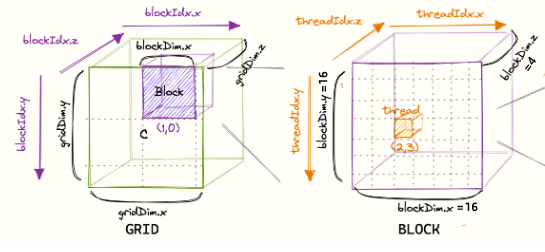
\includegraphics[width=0.5\textwidth]{assets/grid_block.png}
    \caption{Grid and Block Dimensions 3D division [1]}
    \label{fig:1}
\end{figure}

After defining the suitable block dimensions as (16, 16, 4), we move up and needed to compute the appropriate grid dimensions for the thread access to ensure that the entire 3D volume is accounted for. The grid dimensions are calculated by dividing the total number of rows/columns/depth by the corresponding block dimensions axis. However, since this division may not result in a whole number, the formula includes an adjustment to ensure full coverage of the data. Specifically, we add the block dimension minus one to the total size before performing integer division:

\begin{equation}
    \begin{aligned}
        \text{Grid dimension} &= \left\lceil \frac{\text{Total size}}{\text{Block size}} \right\rceil \\
        &\quad = \frac{\text{Total size} + \text{Block size} - 1}{\text{Block size}}
    \end{aligned}
\end{equation}
\\

So for our 3D grids and blocks, the grid dimensions for example the rows kernel become the following:
\begin{equation}
    \begin{aligned}
        \text{row\_grid} = \Bigg( 
        \left\lceil \frac{\text{rows} + \text{blockDim.x} - 1}{\text{blockDim.x}} \right\rceil, \\
        \left\lceil \frac{\text{cols} + \text{blockDim.y} - 1}{\text{blockDim.y}} \right\rceil, \\
        \left\lceil \frac{\text{depth} + \text{blockDim.z} - 1}{\text{blockDim.z}} \right\rceil
        \Bigg)
    \end{aligned}
\end{equation}

Now that the thread access structure has been defined, we can examine the kernels themselves and their implementation. Each kernel primarily needs to identify which part of the volume it will process based on the thread and block indexes. The kernels first determines the specific row, column, and depth indexes that the current thread needs to access in the volume. It then verifies that these indexes are within bounds; if they are out of bounds, the kernel skips any transformation entirely. Once the bounds are validated, the kernel performs the logic associated with the 1D DWT operation along the respective dimension. This involves calculating the sum of the low and high components, which are then stored back into their respective positions in the volume, adhering to the flattened row-major order. Within the kernels there are two float pointers to device memery. One for the data to be worked on and one for the tempory output data. 

Outside the kernels, in the 'dwt 3d' fucntion these pointers are swapped after each kernel call to ensure that the data sequence happens correctly and the next dimension must work off the result of the previous. Finally after the 1d dwt kernels we need a kernel to map the volume back to the original order. Using the same block dimension the map kernel simply maps the data back to the original order by using the thread index. Note this mapping function was initally created when the multi-level function was going to be implemented. However, it was kept in the final implementation as it ensured that the transfer of the transformed data back to the original order was done correctly. The exess tempory volume is freed and the following memory is returned to the host.
 

\section{1.d Effective Use Of Advanced Facilities}

This section is concerned with the methods in which the optimizations of the implementation was achieved with resepct to CUDA facilities. The main factor investigated here was that of the memory hierarchy. After loading the volume from the binary file the next step is to port any necessary memory needed by the kernels to the device. This is handled in the 'toGPU' function.

We have two main tpyes of memeory to be transfered, the 3d volume and the filter low and high coefficients. The filter low and high coefficients are kept hard coded in the 'assignment.cu' file as 2d vectors where the db number determines which vector of coeffs must be given. These coeffs must be transfered to the device memory since they are part of the convolution. Two most effective methods of transfer and access where explored, shared memory and constant memory.

The shared memory initilization of the low and high coefficients involved having two additional float pointer on top of the volume pointer to device memeory. In the 'toGPU' function the low and high coefficients are fetched using the respective db number, memory is allocated for the pointers using 'cudaMalloc' and coefficients coppied to gloabl memory using 'cudaMemcpy'. So shared memory is initally declared in gloabl memory but then within the kernels the shared memory is defined and local threads on the same block can access the shared memory at a much faster rate than global memory. 

The constant memory on the other hand involved having the low and high coefficients declared as constant memory in the kernel file so that they are accessable. In the 'toGPU' function no memor allocation is needed but rather we use 'cudaMemcpyToSymbol' to copy the coefficients to the constant memory. The constant memory is read only and is cached on the device. Allowing each threaded kernel to access the constant memory at a much faster rate than global memory.

Each implementation was analysed with the NVIDIA profiler, with the main concerns being the time taken to transfer the data to the device and the effects in the kernels due to data access. It must be noted that during the profiling implementations, initilization timings for cuda where obscuring the timings of inital 'cudaMalloc' or 'cudaMemcpyToSymbol'. 

\begin{figure}[h]
    \centering
    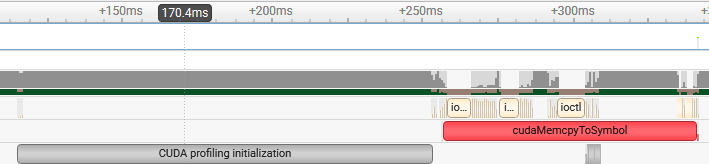
\includegraphics[width=0.5\textwidth]{assets/blaimed-mem.png}
    \caption{cudaMemcpyToSymbol blaimed for initalization time}
    \label{fig:2}
\end{figure}

\begin{figure}[h]
    \centering
    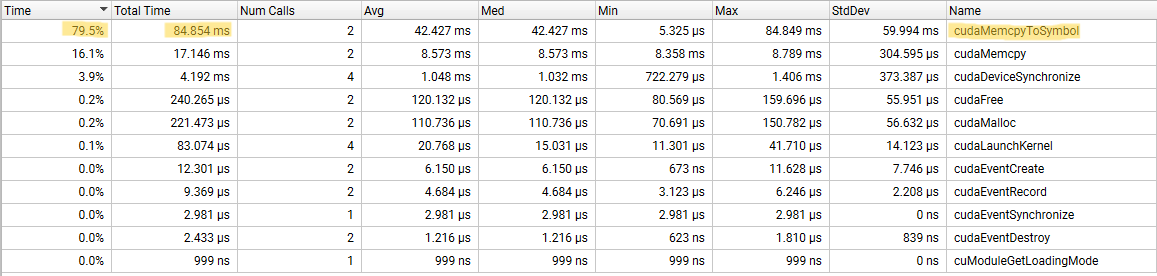
\includegraphics[width=0.5\textwidth]{assets/blaimed-mem-sum.png}
    \caption{Summary showing abnormally high cudaMemcpyToSymbol time}
    \label{fig:3}
\end{figure}

That is since they where the first cuda calls the profiler was blaiming them for the initalization time. So instead additional cudaEvents where added to the code to measure the time taken for the memory transfer. These where then also blaimed for the initalization time. Allowing us to see the actual time taken for the memory transfer.


\begin{figure}[h]
    \centering
    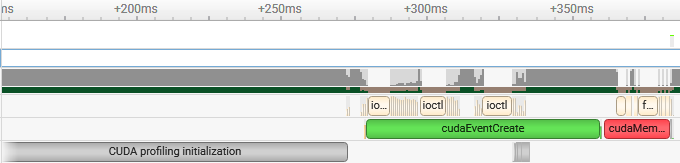
\includegraphics[width=0.5\textwidth]{assets/blaimed-event.png}
    \caption{cudaEvent blaimed for initalization time}
    \label{fig:4}
\end{figure}

\begin{figure}[h]
    \centering
    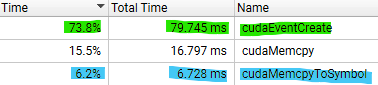
\includegraphics[width=0.5\textwidth]{assets/blaimed-event-sum.png}
    \caption{Summary showing blaimed time moved to cudaEvent}
    \label{fig:5}
\end{figure}

Since the blaiming issue is resolved and we know why our results initially seemed to be obscured by so much we can foucs back on the comparision between shared memory and constant memory. Each case will be analysed with the NVIDIA profiler and confiremd with a cudaEvent record of the time taken for the both the memory transfer and the kernel execution.

\begin{figure}[h]
    \centering
    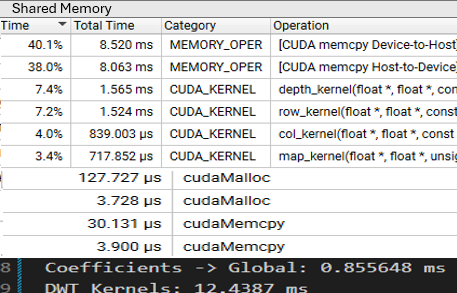
\includegraphics[width=0.5\textwidth]{assets/shared-prof.png}
    \caption{Shared Memory Profiling Results}
    \label{fig:6}
\end{figure}

\begin{figure}[h]
    \centering
    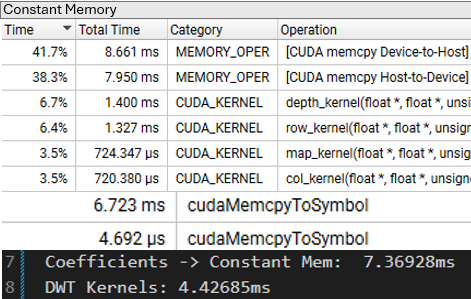
\includegraphics[width=0.5\textwidth]{assets/const-prof.png}
    \caption{Constant Memory Profiling Results}
    \label{fig:7}
\end{figure}

\section{Conclusion}
Conclude your report here.

\appendices
\section{Appendix Title}
Appendix text goes here.

\section*{Acknowledgment}
The authors would like to thank...

\begin{thebibliography}{1}

\bibitem{IEEEhowto:kopka}
H.~Kopka and P.~W.~Daly, \emph{A Guide to \LaTeX}, 3rd~ed. Harlow, England: Addison-Wesley, 1999.

\end{thebibliography}

\end{document}